\iffalse
\documentclass[journal,12pt,twocolumn]{IEEEtran}
\usepackage{cite}
\usepackage{amsmath,amssymb,amsfonts,amsthm}
\usepackage{algorithmic}
\usepackage{graphicx}
\usepackage{textcomp}
\usepackage{xcolor}
\usepackage{txfonts}
\usepackage{listings}
\usepackage{enumitem}
\usepackage{mathtools}
\usepackage{float}
\usepackage{gensymb}
\usepackage{comment}
\usepackage[breaklinks=true]{hyperref}
\usepackage{tkz-euclide} 
\usepackage{listings}
\usepackage{gvv}                                        
\def\inputGnumericTable{}                                 
\usepackage[latin1]{inputenc}                                
\usepackage{color}                                            
\usepackage{array}                                            
\usepackage{longtable}                                       
\usepackage{calc}            
\usepackage{multirow}                                         
\usepackage{hhline}                                           
\usepackage{ifthen}                                           
\usepackage{lscape}
\usepackage{amsmath}
\newtheorem{theorem}{Theorem}[section]
\newtheorem{problem}{Problem}
\newtheorem{proposition}{Proposition}[section]
\newtheorem{lemma}{Lemma}[section]
\newtheorem{corollary}[theorem]{Corollary}
\newtheorem{example}{Example}[section]
\newtheorem{definition}[problem]{Definition}
\newcommand{\BEQA}{\begin{eqnarray}}
\newcommand{\EEQA}{\end{eqnarray}}
\newcommand{\define}{\stackrel{\triangle}{=}}
\theoremstyle{remark}
\newtheorem{rem}{Remark}

\begin{document}

\bibliographystyle{IEEEtran}
\vspace{3cm}

\title{NCERT Discrete - 11.9.3.11}
\author{EE23BTECH11037 - M Esha$^{*}$}

\maketitle
\newpage
\bigskip

\renewcommand{\thefigure}{\theenumi}
\renewcommand{\thetable}{\theenumi}

\vspace{3cm}
\textbf{Question 11.9.3.11:}

Evaluate $\sum_{k=1}^{11} (2 + 3^k)$.

\solution
\fi
\begin{table}[h!]
  \centering
  \begin{tabular}{|c|c|c|}
   \hline
   variable&value&description \\
   \hline
   $x(0)$ & $5$ & first term \\
   \hline
   $r$ & $3$ & common ratio of the GP\\
   \hline
   $x(n)$ & $2+3^{n+1}u\brak{n}$& $n^{th}$ term \\
   \hline
\end{tabular}


  \caption{Input Parameters}
    \label{tab:eshatable1}
\end{table}\\

\begin{align}
x\brak{n} &= \brak{2+3^{n+1}}u(n)\\
x\brak{n} &= \brak{2+3^{n}\cdot{3}}u(n)\\
X\brak{z} &= \frac{2}{\brak{1-z^{-1}}}+\frac{3}{\brak{1-3z^{-1}}} , \quad |z|>3\\
y\brak{n} &= x\brak{n}*u\brak{n} \\
Y\brak{z} &= X\brak{z}U\brak{z}\\
&=\frac{2}{\brak{1-z^{-1}}^{2}}+\brak{\frac{3}{\brak{1-3z^{-1}}\brak{1-z^{-1}}}} ,\quad |z|>3
\end{align}
 Using Contour Integration to find the inverse $Z$-transform,
\begin{align}
y(n)&=\frac{1}{2\pi j}\oint_{C}Y(z) \;z^{n-1} \,dz  \\
y(10)&=\frac{1}{2\pi j}\oint_{C}\brak{\frac{2z^{9}}{\brak{1-z^{-1}}^{2}}+\frac{3z^{9}}{\brak{1-3z^{-1}}\brak{1-z^{-1}}}} \, dz\\
&=\frac{1}{2\pi j}\oint_{C}\brak{\frac{2z^{9}}{\brak{1-z^{-1}}^{2}}+\frac{3}{2}\brak{\frac{z^{11}}{z-3}-\frac{z^{11}}{z-1}}} \,dz\\
R &=\frac{1}{\brak {m-1}!}\lim\limits_{z\to a}\frac{d^{m-1}}{dz^{m-1}}\brak {{(z-a)^{m}}f\brak{z}}
\end{align}
For $R_1$ , $m=2$ :
\begin{align}
R_1 &=\frac{1}{\brak {1}!}\lim\limits_{z\to 1}\frac{d}{dz}\brak {{\brak{z-1}^{2}}\frac{2z^{11}}{{\brak{z-1}^2}}}  \\
&=2\lim\limits_{z\to 1}\frac{d}{dz}(z^{11})   \\
&=22
\end{align}
For $R_2$ , $m=1$:
\begin{align}
R_2 &=\frac{1}{\brak {1-1}!}\frac{3}{2}\lim\limits_{z\to 3}\brak{\brak{z-3}\frac{z^{11}}{\brak{z-3}}} \\
&=\frac{3}{2}\cdot{3^{11}}  \\
&=265720.5
\end{align}
For $R_3$ , $m=1$ :
\begin{align}
R_3 &=\frac{1}{\brak {1-1}!}\frac{3}{2}\lim\limits_{z\to 1}\brak{\brak{z-1}\frac{z^{11}}{\brak{z-1}}} \\
&=\frac{3}{2}\lim\limits_{z\to1}z^{11}\\
&=\frac{3}{2}\\
 R_1 + R_2 - R_3 &= 265741\\
    \implies  y{(10)} &= 265741
\end{align}
\begin{figure}[b]
    \centering
    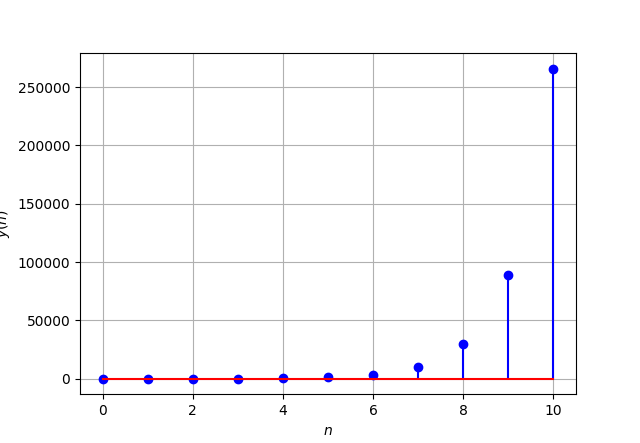
\includegraphics[width=\columnwidth]{ncert-maths/11/9/3/11/figs/fig1.png}
    \caption{stem plot }
    \label{fig:eshaplot1}
\end{figure}
%\end{document}
